% \documentclass{standalone}
\documentclass{scrreprt} % comment this out when done editing
\usepackage{chez}

\begin{document}

\section{Unit 1}

\subsection{August 18, 2021}

\subsubsection{Mr. Clifford's Introduction Video}

\begin{itemize}
	\item Scarcity is the idea that there are limited resources.
	\item Example: Thursday night flight for \$275, \$300, \$325 dollar
	flight. The most expensive flight was actually the cheapest because of
	opportunity cost: she could work at the restaurunt for the next few days.
	\item Why don't we produce all the phones in our country?
	\item Unseen costs: because of costs in the United States, phones are
	much cheaper because China manufacturing is significantly cheaper in the
	United States. Economists often oppose tarriffs for this reason.
\end{itemize}

\begin{definition}[Economics 1]
	The study of how people interact with each other and with their natural
	surroundings in producing their livelihoods, and how this changes over time.
\end{definition}

\begin{definition}[Economics 2]
	Economics is about how individuals, businesses, governments, and nations
	make choices about how to allocate limited resources when faced with
	unlimited wants and needs.
\end{definition}

In essence, economics solves the problme of scarcity - which occurs when there
are limited quantities of things.

\begin{definition}[Resources]
	Anything that can be used to produce something else.
\end{definition}

\subsubsection{The Factors of Production}

\begin{itemize}
	\item Labor: the time and effort that people devote to producing goods
	and services.
	\begin{itemize}
		\item Human capital: the knowledge and skill base of workers in society
		from education, trainings, and experience.
		Investing in human capital can increase your productive capacities as
		an economy. McDonald's and many companies will pay for associated colleges.
	\end{itemize}
	\item Capital: Items used to produce goods and servies: machines, tools,
	buildings. NOT: money, stocks.
	\item Land: Nature that we use to produce goods and services: water, animals, minerals
	\item Entrepreneurship: resource that decides how to organize the land, labor.
	and capital of production; makes decisions and bears risks.
\end{itemize}

\begin{remark}
	Technology falls under capital, since it is able to produce goods and services.
	In the future, this may fall under its own category because they are able
	to produce larger things.
\end{remark}

\subsubsection{How does scarcity impact human behavior?}

People must make choices about how to use scarce resources.

\begin{definition}[Tradeoffs]
	All alternatives that are considered when making a choice.
\end{definition}

\begin{definition}[Opportunity Cost]
	The value of the next best alternative when making a decision.
\end{definition}

Example: by watching a movie at home instead of going out with friends, you are trading
the benefits of added stress of going outdoors.

How do individuals make the best decisions?

\begin{itemize}
	\item Benefits: the added satisfaction and benefit when a good is purchased.
	\item Costs: The added costs (and opportunity costs) when a good is purchased.
\end{itemize}

\subsubsection{Should a city host the olympics?}

\begin{itemize}
	\item How are the land, labor, capital, and entrepeneurship used if
	you host the olympics.
	\begin{itemize}
		\item Venues cost \$ 7.6 billion. Bids are usually an optimistic estimate.
		\item One year postpoponent meant that there were many costs added.
		\item New costs are added incurred around 2.5 billion dollars to the games' budget.
		\item COVID also is taking away ability to recoup that money.
		; There will be no income from visitors because of COVID.
		\item Around 2 billion dollars lost in economic benefits.
		\item Corporate sponsors contribute billions of dollars and the IOC
		committed around 600 million. The overall cost of the pandemic is much
		higher than the olympics.
		\item Japan has spent over 800 billion dollars on stimulus packages.
	\end{itemize}
	\item What's something interesting you heard?
	\begin{itemize}
		\item First game to be postponed.
		\item Most expensive summer game ever.
		\item Cost over 20 billion by the end.
	\end{itemize}
	\item What are the trade-offs of hosting?
	\begin{itemize}
		\item You often lose money.
		\item There would be no spectators this year because of COVID-19.
	\end{itemize}
\end{itemize}

\subsection{August 23, 2021}

Discuss what your terms mean, adn then come up with a group motion to represent
this term.

\begin{enumerate}
	\item Economics
	\item Scarcity
\end{enumerate}

\subsection{August 24, 2021}

\subsubsection{Notes}

How do you model scarcity on a curve.

\begin{definition}[Production Possibilities Curve]
	A curve that shows the maximum combinations of goods and services
	that can be produced, given the fixed factors of production (scarcity).
	Shows: Trade-off, efficiency, inefficiency, opportunity costs, and growths or contractions.

	Consumer goods vs capital goods. The x-axis is the capital goods, and the
	y-axis is the consumer goods. Those on the outside of the curve are unattainable.

	PPC Features:

	\begin{itemize}
		\item The model shows the two alternative choices someone or a country
		can make.
		\item Because scarcity exists, there is a maximum amount of goods and
		services that can be produced.
	\end{itemize}
	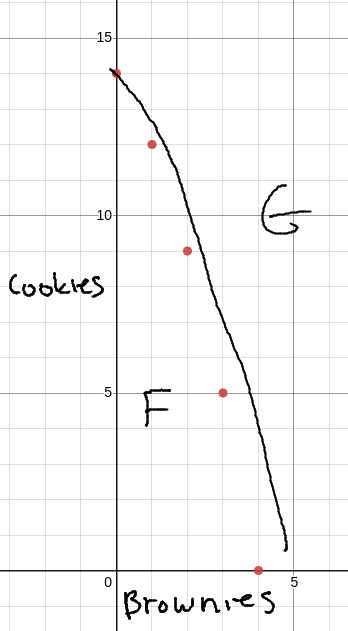
\includegraphics[scale=0.4]{2021-08-24-13-20-08.png}
	
	Note that any points that lie inside of the curve are inefficient.
	In order to calculate the opportunity cost, we calculate from moving points:

	\textbf{Opportunity Costs}

	\begin{itemize}
		\item A to B: gain one brownie and give up two cookies.
		\item D to C: lose one brownie and gain four cookies.
		\item E to B: lose three brownies and gain twelve cookies.
		\item A to E: gain four brownies and give up fourteen cookies.
	\end{itemize}
\end{definition}

\subsubsection{Homework}

Day 1: Review: Answer a few term-based questions before diving into today’s content.

\begin{enumerate}

\item What is the basic problem of economics? Explain this term.

Scarcity. There is a limit to how much something can be produced, or exist.
As a result, distribution of resources is a problem.

\item Why would economists say there is no such thing as a free lunch? 

There is no such thing as a free lunch. The free lunch is a false
statement. This is because some labor is required to produce a good, and all
goods in lunch require some labor.

\item What does the Production Possibilities Curve show? What resources are fixed?

The Production Possibilities Curve shows the trade-offs between two
alternatives. The resources that are fixed are the summation of the alternatives
being considered.

\item How does the curve show scarcity?

The curve shows scarcity because as the amount of one good is increased, the
amount of the other good is decreased, implying that there is a finite amount.

\item Plot
\item Star

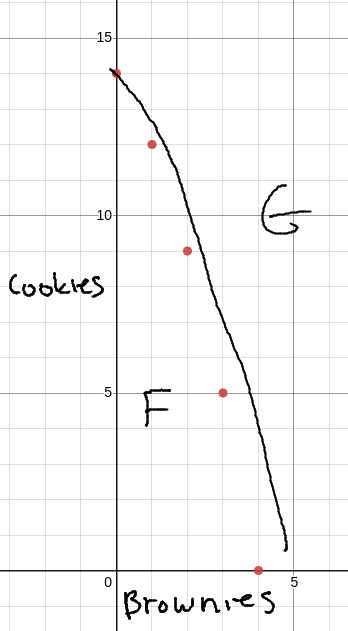
\includegraphics[scale=0.4]{2021-08-24-13-20-08.png}

\item Calculate the opportunity cost of the following points:

\begin{itemize}
	\item A to B: gain one brownie and \textbf{give up two cookies}.
	\item D to C: \textbf{lose one brownie} and gain four cookies.
	\item E to B: \textbf{lose three brownies} and gain twelve cookies.
	\item A to E: gain four brownies and \textbf{give up fourteen cookies}.
\end{itemize}

\item Since the graph looks relatively linear, the opportunity cost looks
constant.

\item What will happen to the PPC for brownies and cookies if… (shift out, shift in, no shift)
\begin{itemize}
	\item There is an increase in technology

	The production curve will shift right because more goods can be produced.

	\item There is a natural disaster, such as a major earthquake
	
	The production curve will shift left because less goods can be produced.

	\item There is high unemployment
	
	The production curve will shift left because less goods can be produced.

	\item There is an improvement in human capital, or education

	The production curve will shift right because more goods can be produced.

\end{itemize}

\item When in history might there have been a time that a country operated at an inefficient point of production?

In the past, people have been at an inefficient point of production. For example,
in the late 1800s, the United States was at an inefficient point of production
because it was using more labor than it could produce. This event is called
the Panic of the 1893.

\end{enumerate}

\subsection{August 25, 2021}

\begin{example}[What's the difference between inefficient pproduction and a contraction?]

\textbf{Inefficient}: a point under the PPC. Indicates an underutilization of resources.
Unemployment, etc.

\textbf{Contraction}: a country has an under-utilization of resources, shifting the curve
leftward or inward. This can occur due to natural disasters.
Ex. natural disaster, war, etc.

\end{example}

What strategies encourage economic growth?

\begin{itemize}
	\item Increasing the quaality of quantity of the factors of production.
	\item Such as land, labor, capital, or entrepeneurship.
	\item Your labor force could become more efficient through education.
	% \item The most important strategy is to increase the amount of labor.
	% \item The second most important strategy is to increase the amount of capital.
\end{itemize}

\end{document}